\documentclass[12pt,a4paper]{article}

% ---------------------------------------------------------------------------
% Versão para a II Semana de Economia Brasileira (CICEF--BNDES).
% Regras de submissão (item 3 -- Apresentação):
%   - até 25 páginas (incluindo gráficos, imagens, referências e anexos)
%   - papel A4, Times New Roman 12, entrelinhas 1,5, margens de 2,5 cm
%   - folha de rosto: título; autor(es) e filiação; resumo (PT e EN);
%     3 a 5 palavras-chave (PT e EN); classificação JEL
%   - citações no formato Chicago (Autor, data, p.), com referências completas
% ---------------------------------------------------------------------------

\usepackage[utf8]{inputenc}
\usepackage[T1]{fontenc}
\usepackage[brazilian]{babel}
\usepackage{newtxtext,newtxmath}   % Times New Roman (texto e matemática)
\usepackage{indentfirst}
\usepackage{setspace}
\usepackage[a4paper,margin=2.5cm]{geometry}
\usepackage{amsmath}
\usepackage{booktabs}
\usepackage{graphicx}
\usepackage{url}
\urlstyle{same}
\renewcommand{\ttdefault}{cmtt}
% Chicago autor-data com vírgula entre autor e ano: (Autor, data, p.)
\usepackage[authoryear,round]{natbib}
\setcitestyle{aysep={,},yysep={;},notesep={, }}
\renewcommand{\bibsection}{\section{\refname}}
\usepackage[dvipsnames]{xcolor}
\usepackage{hyperref}
\hypersetup{hidelinks}

\onehalfspacing

\begin{document}
\thispagestyle{empty}

\begin{center}
{\large\bfseries Formalidade, Composição e Desigualdade no Mercado de Trabalho de Roraima\par}

\vspace{0.8cm}
\begin{singlespace}
Yuri Cesar de Lima e Silva\footnote{SEPLAN/RR e Universidade Federal de Roraima (UFRR).}\par
Andrei de Lima e Silva\footnote{Universidade Federal de Roraima (UFRR).}\par
Jádila Andressa Gomes da Silva\footnote{SEPLAN/RR.}
\end{singlespace}
\end{center}

\vspace{0.4cm}

\begin{singlespace}
\noindent\textbf{Resumo}

\noindent Este artigo analisa como formalidade, gênero e raça/cor se associam aos
diferenciais de rendimento no mercado de trabalho de Roraima, utilizando
microdados da PNAD Contínua de 2016 a 2025. A formalidade permanece associada
a maiores rendimentos após controles extensos. A escolaridade opera em sentidos
opostos: mascara a desvantagem condicional feminina, mas responde por parcela
importante dos elevados \textit{gaps} raciais brutos. Entre trabalhadores formais, os
maiores diferenciais raciais estão fortemente concentrados no setor público.
Para indígenas, a desvantagem permanece relevante, embora gênero e pertencimento
indígena não se acumulem de forma simplesmente aditiva.

\medskip
\noindent\textbf{Palavras-chave:} Formalidade; Diferenciais de rendimento;
Gênero; Desigualdade racial; Roraima.

\bigskip
\noindent\textbf{Abstract}

\noindent This article examines how formality, gender, and race/color are associated
with earnings differentials in Roraima's labor market using Brazilian
Continuous National Household Sample Survey data from 2016 to 2025.
Formality remains associated with higher earnings after extensive controls.
Education operates in opposite directions: it masks women's conditional
disadvantage but accounts for an important share of large raw racial gaps.
Among formal workers, the largest racial differentials are strongly
concentrated in the public sector. Indigenous workers remain disadvantaged,
although gender and Indigenous status do not combine in a simply additive way.

\medskip
\noindent\textbf{Keywords:} Formality; Earnings differentials; Gender; Racial inequality;
Roraima.

\bigskip
\noindent\textbf{Classificação JEL:} J31, J46, J71, J45.
\end{singlespace}

\newpage

\section{Introdução}
\label{sec:introducao}

A formalidade constitui uma das principais dimensões de organização do mercado de trabalho 
brasileiro. O vínculo formal está associado a direitos trabalhistas, previdenciários e 
mecanismos de proteção social, mas também a diferenças relevantes de remuneração. Ainda 
assim, o diferencial observado entre trabalhadores formais e informais não pode ser 
interpretado diretamente como retorno causal à formalização. Diferenças de composição, 
seleção e alocação entre trabalhadores e postos contribuem para o diferencial formal–informal, 
ao mesmo tempo em que diferenças condicionais podem persistir entre trabalhadores 
observavelmente semelhantes \citep{ulyssea2006, curi2006, meghir2015, ulyssea2018}.

A composição também é central para os diferenciais de gênero e raça/cor, embora não 
necessariamente opere da mesma forma entre os grupos. Características educacionais 
relativamente favoráveis às mulheres podem mascarar diferenciais condicionais de 
rendimento, enquanto desigualdades educacionais, segregação ocupacional e alocação 
entre posições remuneratórias contribuem para os \textit{gaps} raciais 
\citep{giuberti2005, soares2000, campante2004, gerard2021}. Para indígenas, a 
evidência latino-americana acrescenta a possibilidade de interação entre desigualdades 
étnicas e de gênero \citep{kolev2015}.

Essa literatura coloca três questões: em que medida os diferenciais de rendimento
refletem composição e seleção, e em que medida permanecem entre trabalhadores com
características semelhantes; se os mecanismos de composição operam da mesma forma para
gênero e raça/cor; e se a entrada no segmento formal está associada à convergência entre
grupos ou se as desigualdades se reorganizam dentro desse segmento. Essas questões são
especialmente relevantes em mercados regionais cuja estrutura produtiva e institucional
difere substancialmente do padrão nacional.

Roraima oferece um contexto particularmente informativo para essa investigação. O estado
combina um mercado de trabalho de pequena escala, elevada presença do setor público e
uma composição demográfica na qual a população indígena possui relevância substantiva.
\citet{moriconi2009} já identificavam Roraima entre os estados com maiores diferenciais
público-privado do país, e estudos posteriores mostram forte heterogeneidade regional e
entre níveis de governo na remuneração do setor público brasileiro
\citep{mattos2022, baez2021}. O período analisado coincide ainda com o influxo
venezuelano, que produziu efeitos heterogêneos sobre diferentes segmentos do mercado de
trabalho de Roraima \citep{ryu2022, santanna2024}; esse processo é tratado aqui como
contexto, e não como mecanismo identificado.

Apesar da extensa literatura sobre informalidade, diferenças de gênero, desigualdade
racial e remuneração pública, essas dimensões são frequentemente analisadas de forma
separada ou a partir de estimativas nacionais e de grandes mercados metropolitanos. Há
menos evidência sobre como formalidade, composição e estrutura institucional se combinam
em um mesmo mercado regional, especialmente quando o setor público representa parcela
elevada do emprego e a categoria indígena pode ser identificada separadamente. A
relevância do caso de Roraima decorre, portanto, da possibilidade de investigar se
regularidades documentadas no mercado de trabalho brasileiro se reproduzem, e por quais
margens, em um ambiente institucional e demográfico particularmente distinto.

Este artigo investiga os diferenciais condicionais de rendimento associados à formalidade,
ao gênero e à raça/cor no mercado de trabalho de Roraima utilizando os microdados da PNAD
Contínua para os quartos trimestres de 2016 a 2025. Estimam-se equações de rendimento
mensal e horário com interações entre formalidade, gênero e raça/cor e controles para
características individuais e inserção ocupacional, incorporando o desenho amostral da
pesquisa. A análise compara ainda uma amostra ampla de ocupados com uma amostra restrita
às relações de emprego e realiza exercícios sobre escolaridade, jornada, setor público e
interseccionalidade.

Os resultados mostram, primeiro, que a formalidade permanece associada a maiores
rendimentos após controles extensos, embora a magnitude do diferencial seja sensível à
composição da amostra e à forma de inserção laboral, em linha com a literatura que
enfatiza a coexistência entre composição, seleção e diferenças condicionais entre
segmentos \citep{curi2006, meghir2015, ulyssea2018}.

Segundo, a escolaridade atua em sentidos opostos na formação dos \textit{gaps} de gênero
e raça/cor. O pequeno diferencial bruto de rendimento por hora entre mulheres e homens
transforma-se em uma desvantagem condicional próxima de 15\% após a inclusão de controles,
sendo a escolaridade decisiva para essa mudança: a maior escolaridade feminina mascara
parte importante do diferencial condicional de gênero, em linha com \citet{giuberti2005}.
Para raça/cor ocorre o movimento oposto: a inclusão da escolaridade reduz
substancialmente os diferenciais de pretos, pardos e indígenas em relação aos brancos,
reforçando o papel das desigualdades educacionais destacado por \citet{soares2000} e
\citet{campante2004}.

Terceiro, a formalidade não está associada a uma convergência generalizada entre os
grupos. O diferencial horário entre homens e mulheres permanece praticamente inalterado
entre trabalhadores formais e informais, e a maior magnitude dos \textit{gaps} raciais
entre trabalhadores formais está fortemente concentrada no setor público, padrão que
dialoga com a literatura sobre alocação desigual dentro do segmento formal e sobre a
heterogeneidade salarial do setor público brasileiro \citep{gerard2021, baez2021}. Por
fim, a separação da categoria indígena revela uma heterogeneidade que tende a desaparecer
em agregações raciais mais amplas. A elevada desvantagem bruta indígena diminui de forma
importante após o controle pela escolaridade, mas um diferencial condicional permanece.
Mulheres indígenas apresentam rendimento inferior ao de homens brancos observavelmente
comparáveis, mas a interação entre gênero e pertencimento indígena indica que as duas
desvantagens não se acumulam de maneira simplesmente aditiva, diferentemente da
evidência de \citet{kolev2015} para o Peru.

O artigo contribui para a literatura em três dimensões: integra formalidade, gênero e
raça/cor em uma mesma estrutura empírica; mostra que uma mesma dimensão composicional
(escolaridade) opera em sentidos opostos na formação dos \textit{gaps} de gênero e
raça/cor; e documenta a centralidade da heterogeneidade dentro do segmento formal em
Roraima, com os maiores diferenciais raciais entre formais concentrados no setor público
e padrões indígenas que seriam ocultados por agregações raciais mais amplas.

Essas contribuições devem ser interpretadas dentro dos limites do desenho empírico.
As estimações não identificam efeitos causais da formalidade, do gênero, da raça/cor
ou do emprego público. Diferenciais residuais podem incorporar características produtivas
não observadas, experiência, qualidade da educação, alocação entre firmas, carreiras e
postos de trabalho, além de mecanismos discriminatórios. O objetivo é caracterizar a
estrutura dos diferenciais condicionais e as dimensões observáveis associadas à sua
composição, sem equiparar coeficientes residuais a discriminação ou retornos causais.

Além desta introdução, a Seção 2 revisa a literatura; a Seção 3 apresenta os dados e a
estratégia empírica; a Seção 4 discute os resultados principais; a Seção 5 examina
mecanismos e heterogeneidades; a Seção 6 apresenta os exercícios de robustez; e a
Seção 7 reúne as considerações finais.

\section{Revisão da literatura}
\label{sec:literatura}

\subsection{Formalidade, seleção e segmentação}

A interpretação dos diferenciais entre trabalhadores formais e informais passou por uma
mudança importante na literatura de economia do trabalho. A visão tradicional de
segmentação admite que trabalhadores com características produtivas semelhantes recebam
remunerações distintas por estarem alocados em segmentos sujeitos a instituições,
barreiras à entrada e estruturas salariais diferentes. A interpretação alternativa
enfatiza seleção e vantagem comparativa: como trabalhadores, firmas e postos são
heterogêneos, o diferencial observado entre formais e informais pode refletir, ao menos
parcialmente, a composição de quem alcança cada posição. \citet{ulyssea2006}, ao
sistematizar a literatura brasileira, mostra que essas interpretações não são mutuamente
exclusivas e que os resultados dependem também da definição de informalidade empregada.

\citet{curi2006} exploram o caráter longitudinal da Pesquisa Mensal de Emprego (PME) e as
transições individuais entre posições formais e informais nas décadas de 1980 e 1990. Ao
controlar características individuais não observadas mediante efeitos fixos, os autores
encontram diferenciais bastante menores que os obtidos em comparações transversais (cerca
de 10\% na década de 1980 e aproximadamente 5\% na de 1990) e interpretam a intensa
mobilidade entre segmentos como evidência contrária a uma segmentação rígida. Um prêmio
formal elevado em regressões de corte transversal não pode, portanto, ser automaticamente
atribuído ao contrato formal.

A conclusão, contudo, depende da forma como heterogeneidade e seleção são tratadas.
\citet{dalberto2018}, utilizando efeitos de tratamento quantílicos sob alocação endógena,
encontram diferenciais favoráveis à formalidade ao longo de grande parte da distribuição,
particularmente elevados entre trabalhadores de menor rendimento. \citet{bargain2011},
comparando Brasil, México e África do Sul, mostram que emprego assalariado informal e
trabalho por conta própria não constituem posições equivalentes, distinção também
presente em estudos brasileiros de escolha ocupacional, como \citet{hirata2010b}. A
pergunta relevante deslocou-se, assim, de ``o mercado é ou não segmentado?'' para
``quais trabalhadores e postos compõem a informalidade e em quais partes do mercado
persistem diferenciais condicionais?''.

Modelos posteriores incorporaram explicitamente essa coexistência de mecanismos.
\citet{meghir2015} desenvolvem um modelo de \textit{search} em equilíbrio, com fricções e
heterogeneidade de trabalhadores e firmas, disciplinado por microdados da PME, no qual
formalidade e informalidade coexistem mesmo entre firmas de produtividade semelhante e os
diferenciais salariais resultam simultaneamente de produtividade, seleção, fricções e
decisões das firmas. \citet{ulyssea2018} distingue firmas inteiramente informais de firmas
formalmente registradas que empregam trabalhadores sem vínculo formal, mostrando que o
segmento informal é internamente heterogêneo. Com a PNAD, uma especificação com controles
individuais e setoriais produz diferencial formal–informal próximo de 29\%, drasticamente
reduzido quando são utilizados dados empregador–empregado e controladas diferenças entre
firmas. Um único coeficiente de formalidade não constitui, portanto, medida de segmentação
nem de retorno causal à formalização, pois combina composição dos trabalhadores, alocação
entre firmas e ocupações, características institucionais e diferenças condicionais
remanescentes. É essa interpretação que orienta, neste artigo, a comparação entre amostras
ampla e restrita e a introdução progressiva de controles por escolaridade, atividade e
ocupação.

\subsection{Gênero, raça e composição dos diferenciais de rendimento}

A literatura sobre diferenciais de gênero e raça compartilha a preocupação em distinguir
diferenças de características das diferenças de remuneração dessas características, mas
os mecanismos de composição não necessariamente operam da mesma forma para os dois grupos.
Utilizando PNAD e a decomposição de Oaxaca para 1981, 1988 e 1996, \citet{giuberti2005}
mostram que as características observáveis das mulheres brasileiras, especialmente sua
maior escolaridade, implicariam rendimentos superiores aos masculinos se fossem
remuneradas segundo a estrutura dos homens; a diferença observada surge porque os retornos
a essas características são distintos entre os grupos.

A evidência posterior reforçou tanto a redução histórica do \textit{gap} quanto sua
persistência. \citet{madalozzo2010}, com PNADs de 1978, 1988, 1998 e 2007 e decomposição
de Oaxaca que incorpora ocupação e atividade, documenta queda do componente não explicado
de aproximadamente 33\% para cerca de 15\%, sem que ele desapareça, além de persistente
segregação ocupacional. Controlar ocupação aproxima trabalhadores em postos semelhantes,
mas pode absorver parte da própria desigualdade se a distribuição entre ocupações fizer
parte do mecanismo de interesse. \citet{morello2021}, com PNADs de 1996 a 2015 e
\textit{propensity-score matching} restrito ao suporte comum entre homens e mulheres,
encontram componente desfavorável às mulheres persistentemente significativo, em torno de
13\%–20\%, com heterogeneidade relevante entre ocupações. Castro et al. (2022) também
encontram persistência de diferenciais femininos no agronegócio brasileiro utilizando
estratégias que consideram seleção e heterogeneidade distributiva.

A literatura racial brasileira identifica um papel muito maior das desigualdades
acumuladas antes da comparação salarial. \citet{soares2000} encontra que parcela
importante da desvantagem de trabalhadores negros está associada às características com
que eles chegam ao mercado de trabalho. \citet{campante2004}, aplicando uma decomposição
inspirada em Oaxaca-Blinder à PNAD de 1996 e comparando Nordeste e Sudeste, mostram que
desigualdades educacionais persistentes reduzem o componente atribuível diretamente ao
mercado de trabalho, mas que permanece uma diferença condicional com intensidade distinta
entre regiões, indicando que resultados nacionais podem ocultar estruturas locais muito
diferentes.

Estudos recentes deslocaram parte da atenção para a alocação dos trabalhadores dentro do
próprio mercado. Usando registros empregador–empregado, \citet{gerard2021} mostram que
trabalhadores não brancos estão menos representados em estabelecimentos que pagam maiores
prêmios salariais, de modo que o \textit{sorting} entre firmas responde por parcela do
diferencial racial, margem que pesquisas domiciliares dificilmente conseguem observar.
\citet{cardoso2025} documentam segregação racial em níveis finos da estrutura ocupacional.
O resíduo de uma equação salarial pode, assim, incorporar discriminação, mas também
alocação entre firmas, tarefas e posições não observadas.

Essa questão é ainda mais sensível para a população indígena. A evidência
latino-americana mostra que diferenças de educação, localização e inserção ocupacional
respondem por parcela relevante dos \textit{gaps} étnicos, mas não necessariamente por sua
totalidade \citep{canelas2014, canedo2019}. Para o Peru, \citet{kolev2015} encontram
desvantagem particularmente intensa para mulheres indígenas, o que motiva investigar
explicitamente como gênero e pertencimento étnico se combinam. A literatura brasileira
ainda é limitada nesse aspecto: \citet{marques2024}, por exemplo, encontram forte
desvantagem do conjunto preto-pardo-indígena entre 2002 e 2015, mas a agregação PPI não
permite identificar se o padrão indígena acompanha o de pretos e pardos, heterogeneidade
que interessa particularmente a estados como Roraima. Em conjunto, essa evidência sugere
que a composição observável não precisa reduzir os \textit{gaps} de gênero e raça na mesma
direção: a escolaridade relativamente elevada das mulheres pode mascarar uma desvantagem
condicional, enquanto a desigualdade educacional racial tende a ampliar o diferencial
bruto.

\subsection{Estrutura regional e setor público}

Uma terceira vertente diz respeito ao setor público. O diferencial público–privado é
elevado em comparações brutas, mas grande parte dele está associada à composição dos
trabalhadores e varia intensamente entre regiões e níveis governamentais.
\citet{foguel2000}, utilizando a PNAD de 1995, mostram que servidores públicos possuem, em
média, características associadas a maiores rendimentos e que a magnitude do diferencial
muda entre União, estados e municípios. \citet{moriconi2009}, analisando as PNADs de 1995
a 2004, identificam Roraima entre os estados com maiores diferenciais público–privado do
país.

\citet{mattos2022}, explorando a estrutura em painel da PNAD Contínua entre 2016 e 2019,
mostram que o diferencial transversal público–privado supera 60\%, mas que o componente
residual é consideravelmente menor quando a heterogeneidade individual é controlada.
\citet{baez2021}, utilizando a PNAD Contínua de 2017 a 2019 e distinguindo níveis de
governo, mostram que os diferenciais são muito superiores no governo federal, menores nos
estados e próximos de zero ou negativos em algumas comparações municipais. Mesmo após
identificar um diferencial associado ao emprego público, parte da heterogeneidade interna
de carreiras, órgãos e níveis de governo continua, portanto, não observada na PNAD
Contínua.

Em síntese, as três vertentes convergem para uma interpretação comum: características
dos trabalhadores, seleção para diferentes formas de inserção, alocação entre ocupações,
firmas e instituições e diferenças de remuneração dentro dessas posições atuam
simultaneamente, e sua importância pode diferir entre gênero e raça e conforme a
estrutura regional. Em um mercado estadual no qual o emprego público possui peso elevado,
diferenças raciais dentro do segmento formal podem refletir não apenas o acesso à carteira
ou ao estatuto, mas também a alocação entre diferentes posições do setor público. É a
partir dessa perspectiva que o artigo combina uma especificação condicional principal com
exercícios sequenciais de composição, compara amostras ampla e restrita, distingue
rendimento mensal e horário e examina separadamente escolaridade, setor público e
interações entre formalidade, gênero e raça/cor.

\section{Metodologia}
\label{sec:metodologia}

\subsection{Dados}
\label{subsec:dados}

A análise utiliza os microdados trimestrais da Pesquisa Nacional por Amostra de
Domicílios Contínua (PNAD Contínua), produzida pelo Instituto Brasileiro de
Geografia e Estatística (IBGE). O recorte principal compreende os quartos
trimestres de 2016 a 2025 para o estado de Roraima. A utilização de um mesmo
trimestre em cada ano busca assegurar maior comparabilidade sazonal entre os
cortes e reduzir a intensidade de reutilização das unidades amostrais decorrente
do esquema rotativo da pesquisa. Como exercício de robustez, a especificação
principal é posteriormente reestimada utilizando os quatro trimestres de
cada ano, com efeitos fixos de ano$\times$trimestre. A estrutura amostral e o
esquema de rotação seguem o desenho oficial da PNAD Contínua
\citep{ibge_pnadc_notas_metodologicas}.

A amostra inicial contém os indivíduos entrevistados em Roraima nos períodos
selecionados. Restringe-se a análise às pessoas com 14 anos ou mais
classificadas como ocupadas na semana de referência e, nas equações de
rendimento, às observações com rendimento positivo e válido no trabalho
principal. A amostra principal, denominada \textit{ampla}, reúne todos os
ocupados para os quais é possível definir a condição de formalidade. Uma segunda
amostra, denominada \textit{restrita}, inclui apenas empregados privados,
trabalhadores domésticos, empregados públicos e militares ou servidores
estatutários, excluindo empregadores, trabalhadores por conta própria e
trabalhadores familiares auxiliares. A distinção permite verificar em que
medida os diferenciais estimados para o conjunto dos ocupados refletem a
heterogeneidade entre formas de inserção laboral, reconhecida na literatura
sobre informalidade \citep{bargain2011,hirata2010b}.

A formalidade é definida a partir da posição na ocupação e, quando pertinente,
do registro do empreendimento. São classificados como formais os empregados
privados e domésticos com carteira, os empregados públicos com carteira e os
militares ou servidores estatutários. Empregados privados, domésticos e públicos
sem carteira são classificados como informais. Entre empregadores e
trabalhadores por conta própria, considera-se formal aquele cujo empreendimento
possui registro no Cadastro Nacional da Pessoa Jurídica (CNPJ) e informal aquele
sem registro. Trabalhadores familiares auxiliares são classificados como
informais. Essa construção incorpora tanto a dimensão contratual da formalidade
entre empregados quanto a dimensão de registro do empreendimento entre
empregadores e trabalhadores por conta própria, em linha com a heterogeneidade
da informalidade discutida por \citet{ulyssea2006} e \citet{ulyssea2018}.

As variáveis dependentes principais são o rendimento mensal real do trabalho
principal e o rendimento real por hora. O rendimento mensal habitual é
deflacionado pelo deflator trimestral oficial da PNAD Contínua. O rendimento por
hora ($w^h_{it}$) é definido por:

\begin{equation}
    w^h_{it}=\frac{w^m_{it}}{4{,}33H_{it}},
    \label{eq:renda_hora}
\end{equation}

\noindent
em que $w^m_{it}$ representa o rendimento mensal habitual e $H_{it}$ as horas
habitualmente trabalhadas por semana no trabalho principal\footnote{O fator 4,33 na equação \ref{eq:renda_hora} resulta de $52/12$ e converte a jornada semanal habitual em uma aproximação da jornada mensal. Dessa forma, o rendimento por hora é obtido dividindo-se o rendimento mensal habitual pelo número estimado de horas habitualmente trabalhadas no mês.}. Nas estimações são
utilizados $\ln w^m_{it}$ e $\ln w^h_{it}$.

A variável de gênero assume valor um para mulheres e zero para homens, que
constituem a categoria de referência. A variável de raça/cor distingue brancos,
pretos, pardos e indígenas, com brancos como referência. A categoria amarela é
excluída das especificações que envolvem raça/cor devido ao número reduzido de
observações. A idade entra em nível e ao quadrado, enquanto a escolaridade é
representada por categorias de nível de instrução. Para controlar a inserção
produtiva, utilizam-se os grandes grupos de ocupação e atividade econômica da
PNAD Contínua. Na especificação principal, essas duas dimensões são combinadas
em células ocupação$\times$atividade. Células com menos de 30 observações foram
agrupadas em uma categoria residual, definida na amostra original e mantida
fixa em todas as réplicas.

Todas as estatísticas e estimações incorporam o desenho amostral complexo da
PNAD Contínua. Como pesos amostrais e estrutura do plano de amostragem devem ser
considerados também na estimação da variância
\citep{lumley2004analysis,lumley2010complex}, utiliza-se o peso principal e os 
pesos de replicação bootstrap disponibilizados pelo IBGE. O desenho é
implementado no pacote \texttt{survey} do R como um
\textit{replicate-weight design}, e as variâncias de coeficientes, contrastes e
efeitos marginais são obtidas a partir dessas réplicas bootstrap.

\subsection{Estratégia empírica}
\label{subsec:estrategia}

A estratégia empírica parte de equações de rendimento de inspiração minceriana
\citep{mincer1974schooling} e busca caracterizar diferenciais condicionais
associados à formalidade, ao gênero e à raça/cor. O desenho não pretende
identificar efeitos causais, uma vez que formalidade, ocupação, atividade e
posição institucional não são aleatoriamente atribuídas. Os parâmetros são,
portanto, interpretados como associações condicionais entre trabalhadores
observavelmente semelhantes \citep{wooldridge2010econometric}.

A especificação principal é

\begin{align}
\ln w_{it}
={}&
\alpha
+\beta_F F_{it}
+\beta_M Mulher_{it}
+\boldsymbol{\beta}_{R}'\mathbf{R}_{it}
+\beta_{FM}(F_{it}\times Mulher_{it})
\nonumber\\
&+
\boldsymbol{\beta}_{FR}'(F_{it}\times\mathbf{R}_{it})
+
\boldsymbol{\beta}_{MR}'(Mulher_{it}\times\mathbf{R}_{it})
+\gamma_1 A_{it}
+\gamma_2 A_{it}^{2}
\nonumber\\
&+
\boldsymbol{\delta}'\mathbf{E}_{it}
+
\boldsymbol{\theta}'\mathbf{C}_{it}
+\lambda_t
+\varepsilon_{it},
\label{eq:modelo_principal}
\end{align}

\noindent
em que $\ln w_{it}$ representa alternativamente o logaritmo do rendimento
mensal real ou do rendimento real por hora; $F_{it}$ indica formalidade; $Mulher_{it}$ indica gênero feminino;
$\mathbf{R}_{it}$ contém indicadores para pretos, pardos e indígenas;
$A_{it}$ representa idade; $\mathbf{E}_{it}$ reúne as categorias de
escolaridade; $\mathbf{C}_{it}$ representa os efeitos fixos das células
ocupação$\times$atividade; $\lambda_t$ corresponde aos efeitos fixos de
período; e $\varepsilon_{it}$ representa o termo de erro, que reúne fatores não observados associados ao rendimento. 
As interações permitem que o diferencial de gênero varie segundo a
formalidade, que os diferenciais raciais sejam distintos entre formais e
informais e que gênero e raça/cor não se combinem necessariamente de forma
aditiva. Não se inclui uma interação tripla entre formalidade, gênero e raça/cor
na especificação principal, preservando parcimônia diante do tamanho reduzido
de algumas células, especialmente entre indígenas.

Para examinar a importância da composição observável, 
são realizados exercícios sequenciais nos quais características demográficas, 
escolaridade, atividade econômica, ocupação$\times$atividade e setor público são
incorporados progressivamente. Esses exercícios constituem uma forma de 
\textit{accounting}, permitindo acompanhar como os diferenciais estimados 
se modificam à medida que diferentes dimensões de composição são acrescentadas 
ao modelo. A estratégia não corresponde a uma decomposição causal ou Oaxaca–Blinder
\footnote{O exercício de \textit{accounting} é preferido porque permite acompanhar diretamente 
como blocos específicos de controles alteram os diferenciais estimados, sem impor a 
decomposição entre componentes ``explicado'' e ``não explicado'' característica de 
Oaxaca--Blinder.}, mas permite avaliar a sensibilidade dos diferenciais à composição 
observável \citep{wooldridge2010econometric}.

Como a equação \eqref{eq:modelo_principal} contém interações, os coeficientes dos
efeitos principais são condicionais às categorias de referência e não
representam, isoladamente, diferenciais médios da população
\citep{brambor2006understanding}. Os resultados substantivos são, portanto,
apresentados por meio de contrastes lineares. Para gênero, os contrastes são
calculados separadamente entre formais e informais e promediados segundo a composição racial 
ponderada da amostra; para raça/cor, os diferenciais em
relação aos brancos são promediados segundo a composição ponderada de gênero
\footnote{Como a especificação contém interações, os contrastes médios 
correspondem a combinações lineares dos coeficientes estimados. Por exemplo, 
entre trabalhadores informais, o diferencial médio de gênero pode ser escrito
como $\Delta_G=\beta_M+\sum_r \pi_r\beta_{M\times r}$,
em que $\pi_r$ representa a participação ponderada do grupo racial $r$ na amostra.
Assim, a média ponderada dos diferenciais entre grupos pode ser expressa como o 
contraste linear $a'\beta$, cuja variância é apresentada na equação seguinte.}. De
forma geral, para um contraste $\Delta=a'\boldsymbol{\beta}$,

\begin{equation}
    \widehat{\mathrm{Var}}(\widehat{\Delta})
    =
    a'\widehat{\mathbf V}a,
    \label{eq:contraste}
\end{equation}

\noindent
em que $\widehat{\mathbf V}$ é a matriz de variância e covariância obtida com o
desenho bootstrap. O procedimento incorpora, portanto, a covariância entre os
parâmetros envolvidos em cada contraste \citep{lumley2010complex}.

A distinção entre rendimento mensal e rendimento por hora permite ainda
investigar o papel da jornada de trabalho. Como

\begin{equation}
    \ln w^m_{it}
    =
    \ln w^h_{it}
    +
    \ln H_{it}
    +
    \ln(4{,}33),
    \label{eq:identidade_jornada}
\end{equation}

\noindent
a estimação da mesma especificação para rendimento mensal, rendimento por hora
e horas trabalhadas implica, para qualquer regressor $k$,
$\widehat{\beta}^m_k=\widehat{\beta}^h_k+\widehat{\beta}^H_k$. A diferença entre
o coeficiente mensal e o horário pode, assim, ser atribuída exatamente, na
escala logarítmica, à jornada. As horas são tratadas como variável dependente
nesse exercício e não como controle da equação principal, evitando bloquear
mecanicamente esse canal.

As equações de rendimento são complementadas por um modelo para acesso à
formalidade. Estima-se um logit no qual a probabilidade de formalização depende
de gênero, raça/cor, idade, escolaridade, efeitos fixos de período e células
ocupação$\times$atividade. O modelo é estimado separadamente nas amostras ampla
e restrita e com o mesmo desenho amostral das equações salariais. Como os
coeficientes do logit não possuem interpretação direta em pontos percentuais,
reportam-se efeitos marginais médios, calculados como mudanças discretas nas
probabilidades previstas e recomputados em cada uma das réplicas bootstrap
\citep{hanmer2013behind}. Esses resultados também são interpretados de maneira
associacional.

Por fim, a centralidade do setor público em Roraima é examinada por extensões
da especificação principal. Na amostra restrita, adicionam-se um indicador de
emprego público e sua interação com formalidade, permitindo distinguir duas
dimensões distintas e conjuntamente associadas ao rendimento. Em exercício
complementar, a dicotomia formal--informal é substituída pela posição detalhada
na ocupação, distinguindo empregados privados, domésticos e públicos com e sem
carteira, militares ou estatutários, empregadores e trabalhadores por conta
própria. Para avaliar se os diferenciais raciais entre trabalhadores formais variam
entre os setores público e privado, estima-se uma especificação que permite
construir contrastes de raça/cor separadamente para trabalhadores formais no
setor privado/doméstico e no setor público. A fragmentação de algumas células, 
sobretudo entre indígenas, limita parametrizações mais desagregadas.

A interação entre mulher e raça/cor presente na equação principal é utilizada
adicionalmente para avaliar a sobreposição dessas dimensões. O termo de
interação indica se o diferencial conjunto de gênero e pertencimento racial
difere daquele que seria obtido pela simples soma dos respectivos coeficientes
na escala logarítmica. Assim como nos demais exercícios, esse resultado
caracteriza heterogeneidade condicional e não identifica um mecanismo causal
específico.

\section{Resultados}
\label{sec:resultados}

Esta seção apresenta os resultados centrais das equações de rendimento e do
modelo de acesso à formalidade. A análise privilegia o rendimento real por hora,
por aproximar de forma mais direta diferenças no preço do trabalho, e utiliza o
rendimento mensal como dimensão complementar. Os resultados correspondem à
especificação principal, que inclui características individuais, efeitos fixos de
período e células ocupação$\times$atividade. A amostra ampla contém 23.938
trabalhadores ocupados com informação válida de rendimento (13.282 informais e
11.132 formais antes da restrição por rendimento), e a amostra restrita às
relações de emprego contém 16.135 observações. Esses números são contagens
amostrais não ponderadas e não devem ser interpretados como estimativas da
composição populacional do mercado de trabalho de Roraima.

\subsection{Formalidade, estrutura do mercado e acesso à formalidade}
\label{subsec:resultados_formalidade}

A formalidade permanece associada a rendimentos mais elevados após o
condicionamento pelas características individuais e pela inserção produtiva.
Na amostra ampla, o contraste médio associado à formalidade corresponde a
aproximadamente 28,9\% no rendimento por hora. Na amostra restrita às relações
de emprego, que exclui empregadores e trabalhadores por conta própria, o
diferencial diminui para aproximadamente 20,9\%
(Figura~\ref{fig:formalidade_amostras}). Parte do diferencial observado na
amostra ampla está, portanto, relacionada à heterogeneidade entre formas de
inserção que ultrapassam a oposição entre emprego com e sem vínculo formal, mas
o diferencial permanece positivo na comparação mais restrita. Esse padrão é
compatível com a literatura que rejeita a interpretação de um único diferencial
formal--informal como retorno do contrato \citep{curi2006, meghir2015, ulyssea2018}.
Na amostra ampla, a variável combina carteira de trabalho e registro do
empreendimento, razão pela qual o resultado é denominado diferencial de
rendimento associado à formalidade; na amostra restrita, a comparação ocorre
entre relações de emprego e aproxima-se do diferencial salarial associado ao
vínculo formal. Em nenhuma das duas situações a estimativa identifica o retorno
causal da formalização.

\begin{figure}[htbp]
    \centering
    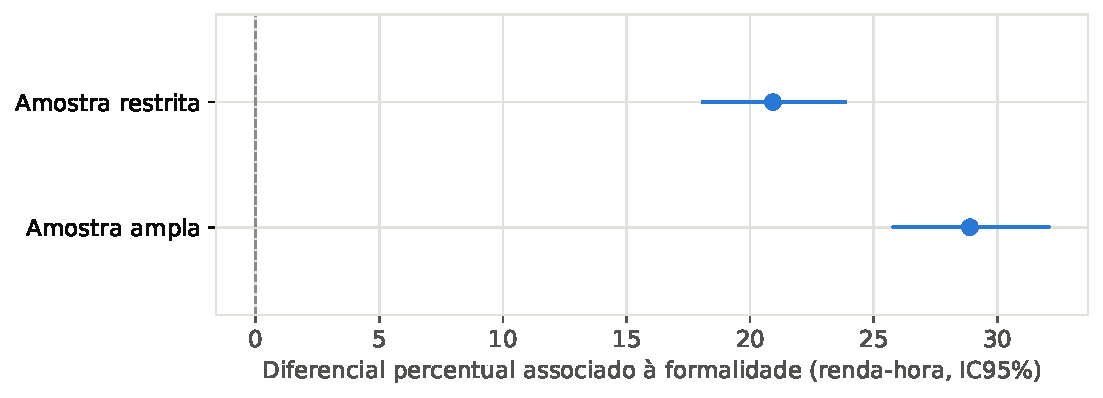
\includegraphics[width=0.72\textwidth]
    {../figures/fig_formalidade_amostras.pdf}
    \caption{Diferencial condicional de rendimento por hora associado à
    formalidade}
    \label{fig:formalidade_amostras}
    \begin{minipage}{0.92\textwidth}
    \vspace{0.2cm}\scriptsize
    \textit{Nota:} Contrastes médios da especificação principal, ponderados pela
    distribuição observada de gênero e raça/cor. Barras representam intervalos
    de confiança de 95\%. A amostra ampla inclui todos os ocupados com condição
    de formalidade definida; a amostra restrita inclui apenas relações de
    emprego. Estimações incorporam o desenho amostral da PNAD Contínua e das
    réplicas bootstrap oficiais do IBGE.
    \end{minipage}
\end{figure}

A existência de um diferencial de rendimento não implica que os grupos
examinados apresentem probabilidades condicionalmente diferentes de alcançar a
formalidade. Na amostra ampla, os efeitos marginais médios do modelo logit
descrito na Seção~\ref{subsec:estrategia} são de $-7,2$ pontos percentuais para
mulheres, $-4,7$ p.p. para pretos, $-2,6$ p.p. para pardos e $-1,9$ p.p. para
indígenas, com erros-padrão de 6,7, 3,8, 2,9 e 4,3 p.p., respectivamente; nenhum
desses contrastes é estatisticamente diferente de zero aos níveis
convencionais. Na amostra restrita, as estimativas também são imprecisas:
$+2,1$ p.p. para mulheres, $-3,8$ p.p. para pretos, $-0,8$ p.p. para pardos e
$-3,6$ p.p. para indígenas, com erros-padrão de 5,0, 4,3, 2,3 e 7,7 p.p.
(Figura~\ref{fig:acesso_formalidade}). Não se detectam, portanto, diferenças
sistemáticas no acesso à formalidade segundo gênero ou raça/cor depois dos
controles observáveis, mas os dados tampouco permitem excluir diferenças
economicamente relevantes. As duas figuras descrevem, assim, margens distintas,
em linha com a cautela da literatura de que diferenças de remuneração entre
posições não implicam, mecanicamente, barreiras observáveis de acesso a essas
posições \citep{ulyssea2006,ulyssea2018}.

\begin{figure}[htbp]
    \centering
    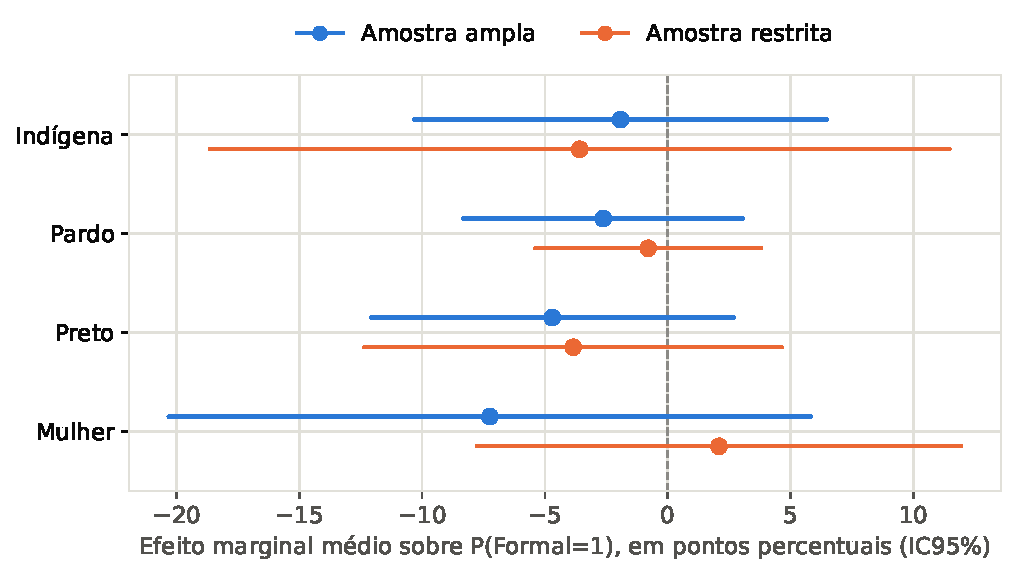
\includegraphics[width=0.78\textwidth]
    {../figures/fig_acesso_formalidade.pdf}
    \caption{Efeitos marginais médios sobre a probabilidade de formalização}
    \label{fig:acesso_formalidade}
    \begin{minipage}{0.92\textwidth}
    \vspace{0.2cm}
    \scriptsize 
    \textit{Nota:} Efeitos marginais médios, em pontos percentuais, do modelo
    logit de acesso à formalidade. As categorias de referência são homem e
    branco. Barras representam intervalos de confiança de 95\%. O modelo inclui
    idade, idade ao quadrado, escolaridade, efeitos fixos de período e células
    ocupação$\times$atividade. Variâncias calculadas com as réplicas
    bootstrap oficiais da PNAD Contínua.
    \end{minipage}
\end{figure}

\subsection{Gênero}
\label{subsec:resultados_genero}

A entrada no segmento formal não está associada a convergência relevante do
rendimento por hora entre mulheres e homens. Como a especificação contém
interações, a comparação substantiva é realizada por contrastes médios
ponderados pela composição racial da amostra, e não pelo coeficiente isolado de
$Mulher_{it}$. O diferencial bruto é pequeno e ligeiramente favorável às
mulheres, em aproximadamente 3,3\%. Na especificação principal, contudo, as
mulheres apresentam rendimento por hora aproximadamente 14,6\% inferior ao dos
homens observacionalmente comparáveis entre informais e 15,0\% inferior entre
formais (Figura~\ref{fig:gaps_genero_raca}, painel a). A diferença entre os dois
\textit{gaps}, de cerca de meio ponto percentual, não é estatisticamente
significativa ($p=0,775$). Dentro da precisão permitida pelos dados, portanto,
não há evidência de que a formalidade esteja associada à redução do diferencial
de gênero no rendimento horário.

A passagem de um diferencial bruto próximo de zero para uma desvantagem
condicional próxima de 15\% indica que a composição observável mascara parte
relevante da desigualdade de gênero, em linha com a literatura que encontra
desvantagens femininas mesmo após controles por capital humano e inserção
ocupacional \citep{giuberti2005, madalozzo2010, morello2021}. Para Roraima,
acrescenta-se que essa diferença condicional é praticamente da mesma magnitude
entre formais e informais. O rendimento mensal apresenta diferença feminina
maior do que o rendimento por hora, o que sugere que o diferencial mensal combina
diferenças na remuneração horária e nas horas trabalhadas; a contribuição de
cada margem é quantificada na Seção~\ref{sec:mecanismos}.

\begin{figure}[htbp]
    \centering
    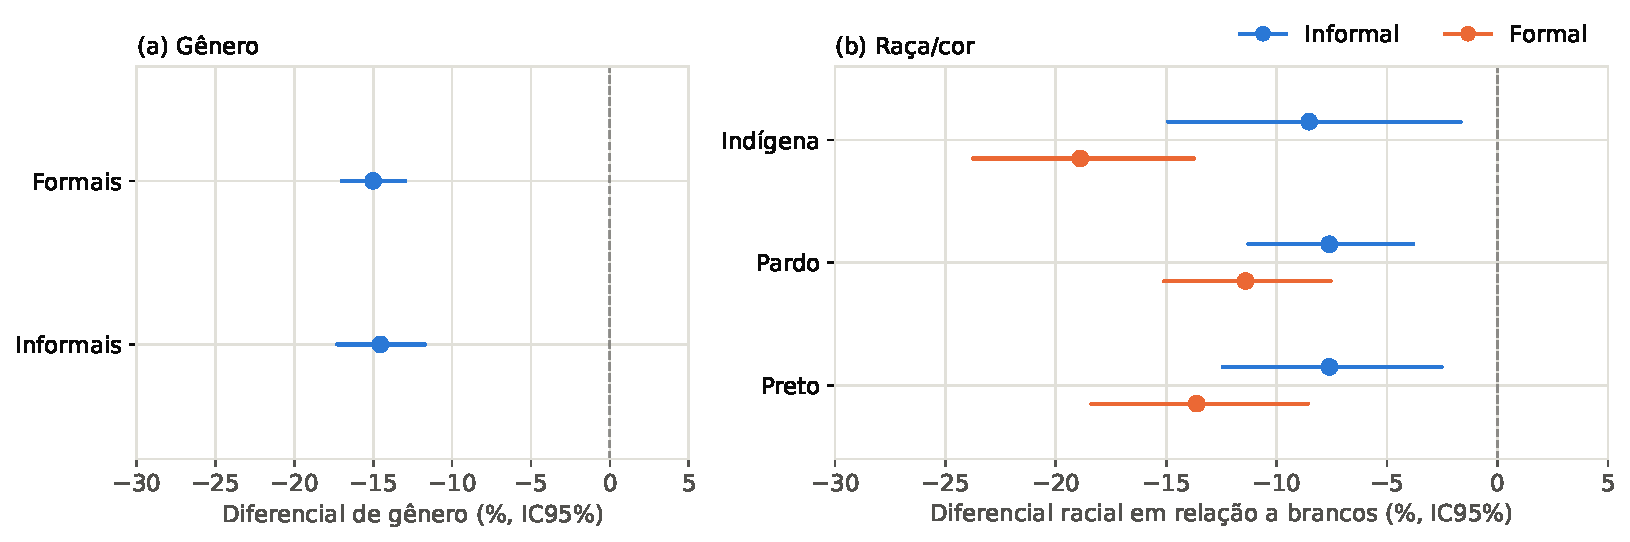
\includegraphics[width=0.88\textwidth]
    {../figures/fig_gaps_genero_raca_formalidade.pdf}
    \caption{Diferenciais condicionais de rendimento por hora, segundo
    formalidade}
    \label{fig:gaps_genero_raca}
    \begin{minipage}{0.94\textwidth}
    \vspace{0.2cm}
    \scriptsize 
    \textit{Nota:} O painel (a) apresenta o diferencial mulher--homem,
    promediado pela distribuição racial da amostra. O painel (b) apresenta os
    diferenciais de pretos, pardos e indígenas em relação aos brancos,
    promediados pela distribuição de gênero. Estimativas provenientes da
    especificação principal na amostra ampla. Barras representam intervalos de
    confiança de 95\%. Valores em porcentagem calculados por
    $100[\exp(\widehat{\Delta})-1]$.
    \end{minipage}
\end{figure}

\subsection{Raça/cor}
\label{subsec:resultados_raca}

Os diferenciais de raça/cor apresentam um padrão distinto. Antes do
condicionamento pelas características observáveis, os diferenciais de
rendimento por hora em relação aos brancos já são expressivos: aproximadamente
$-30\%$ para pretos, $-27\%$ para pardos e $-40\%$ para indígenas. Após os
controles da especificação principal, os \textit{gaps} diminuem
consideravelmente, mas permanecem negativos. Entre informais, os contrastes
médios são de aproximadamente $-7,6\%$ para pretos, $-7,6\%$ para pardos e
$-8,5\%$ para indígenas; entre formais, de $-13,6\%$, $-11,4\%$ e $-18,9\%$,
respectivamente (Figura~\ref{fig:gaps_genero_raca}, painel b). A diferença entre
os \textit{gaps} formal e informal é de aproximadamente $-6,5\%$ para pretos
($p=0,071$), $-4,1\%$ para pardos ($p=0,152$) e $-11,3\%$ para indígenas
($p=0,010$). Há evidência estatisticamente clara, portanto, de ampliação do
diferencial indígena no segmento formal; para pretos, a diferença alcança apenas
significância ao nível de 10\%; para pardos, não se rejeita igualdade entre os
\textit{gaps} nos dois segmentos.

A forte redução entre os diferenciais brutos e condicionais indica que a
composição observável está associada a parcela importante da desigualdade
racial, movimento oposto ao observado para gênero e consistente com
\citet{soares2000} e \citet{campante2004}. A permanência de diferenças após os
controles mostra, contudo, que a composição individual observada não esgota o
diferencial racial. Como desigualdades podem persistir dentro do segmento formal
por meio da alocação não aleatória de trabalhadores entre firmas e posições
\citep{gerard2021}, o maior \textit{gap} observado entre formais não deve ser
interpretado automaticamente como uma característica da formalidade em si; a
Seção~\ref{sec:mecanismos} examina, nesse sentido, o papel do setor público. Os
indígenas, por fim, exibem o maior diferencial nas comparações bruta e
condicional e a maior alteração entre os segmentos formal e informal, o que
reforça a limitação de agregações raciais mais amplas
\citep{canelas2014, canedo2019, kolev2015}.

\section{Mecanismos e heterogeneidades}
\label{sec:mecanismos}

Esta seção investiga quais dimensões observáveis estão associadas a dois padrões
da seção anterior (a trajetória oposta dos diferenciais de gênero e raça/cor com
a inclusão de controles e os maiores \textit{gaps} raciais entre trabalhadores
formais), sem atribuir interpretação causal aos exercícios.

\subsection{Composição e jornada}
\label{subsec:composicao_jornada}

A Figura~\ref{fig:accounting_genero_raca} apresenta os exercícios sequenciais de
\textit{accounting}. No painel (a), o diferencial bruto de rendimento por hora,
de cerca de 3,3\% a favor das mulheres, praticamente não se altera com a
inclusão de idade e idade ao quadrado. A mudança ocorre com a escolaridade: após
sua inclusão, o diferencial passa para aproximadamente $-16,4\%$ e permanece
próximo desse patamar quando são acrescentados controles por atividade,
ocupação$\times$atividade e setor público. A composição educacional relativamente
favorável das mulheres mascara, portanto, parcela importante da desigualdade
condicional de rendimento, padrão coerente com \citet{giuberti2005} e com a
persistência do diferencial documentada por \citet{madalozzo2010} e
\citet{morello2021}.

O painel (b) revela o movimento oposto para raça/cor. Os diferenciais,
próximos de $-30\%$ para pretos, $-27\%$ para pardos e $-40\%$ para indígenas
antes dos controles educacionais, caem para aproximadamente $-13\%$, $-12\%$ e
$-19\%$, respectivamente, após a inclusão da escolaridade; os controles
posteriores produzem alterações comparativamente menores. A escolaridade opera,
assim, em sentidos opostos na formação dos \textit{gaps}: a vantagem educacional
feminina oculta parte da desvantagem condicional das mulheres, enquanto a
desvantagem educacional racial amplia os diferenciais brutos, em linha com o
papel atribuído por \citet{soares2000} e \citet{campante2004} às desigualdades
de qualificação acumuladas antes da comparação salarial. A permanência de
\textit{gaps} após esses controles mostra que a desigualdade racial não se esgota
nessa margem.

\begin{figure}[htbp]
    \centering
    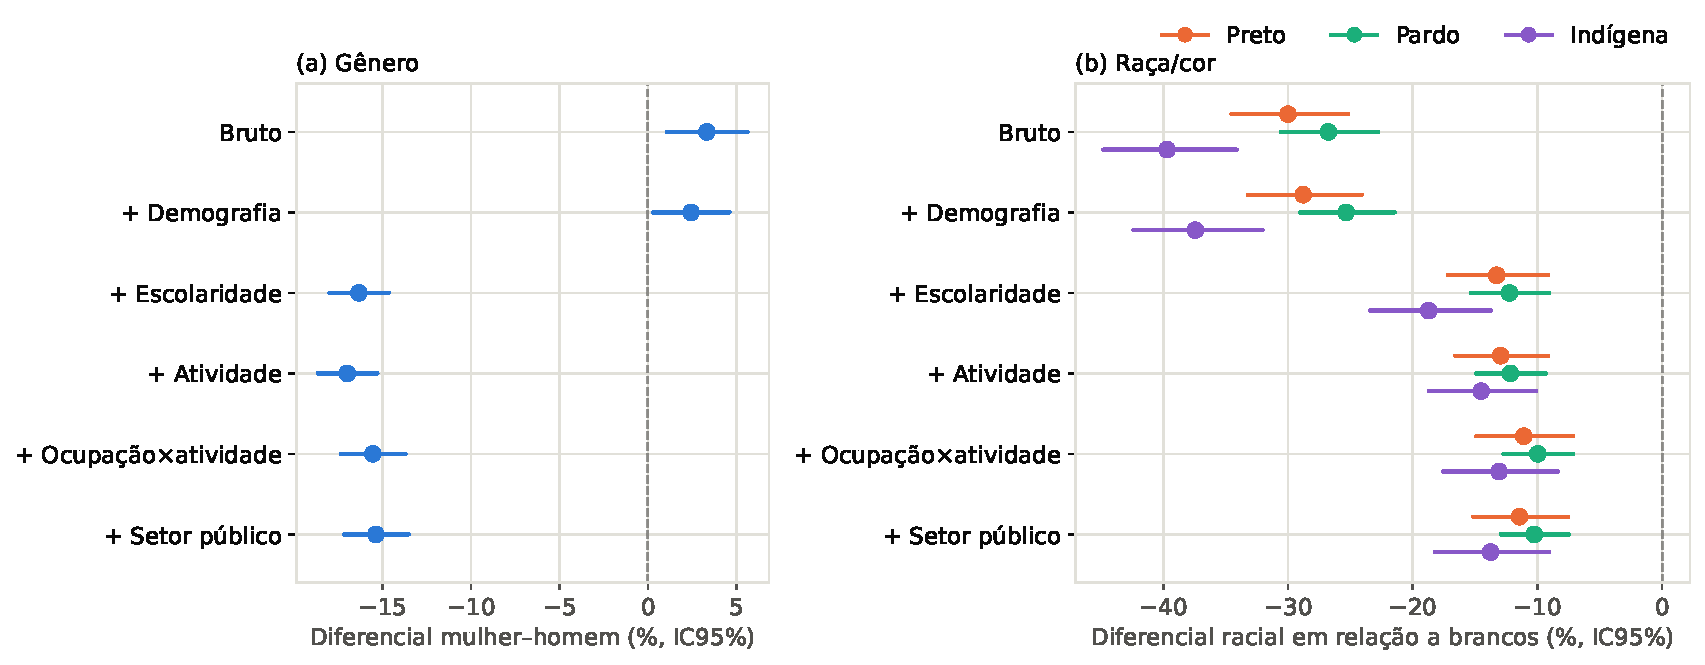
\includegraphics[width=0.88\textwidth]
    {../figures/fig_accounting_genero_raca.pdf}
    \caption{Composição observável dos diferenciais de gênero e raça/cor}
    \label{fig:accounting_genero_raca}
    \begin{minipage}{0.94\textwidth}
    \vspace{0.2cm}
    \scriptsize
    \textit{Nota:} O painel (a) apresenta o diferencial mulher--homem no
    rendimento real por hora à medida que blocos de controles são incorporados
    sequencialmente. O painel (b) apresenta os diferenciais de pretos, pardos e
    indígenas em relação aos brancos segundo a mesma lógica. Estimações para a
    amostra ampla, incorporando o desenho amostral e as réplicas bootstrap
    oficiais da PNAD Contínua. Valores percentuais calculados por
    $100[\exp(\widehat{\beta})-1]$.
    \end{minipage}
\end{figure}

A diferença entre rendimento mensal e horário acrescenta uma segunda dimensão.
A decomposição exata apresentada na metodologia mostra que cerca de 54\% do
diferencial mensal associado ao gênero, na escala logarítmica, decorre de
diferenças na jornada: mulheres trabalham, condicionalmente, cerca de 16,7\%
menos horas semanais do que homens comparáveis. Para raça/cor, aproximadamente
73\%--77\% dos diferenciais mensais estão associados ao componente de
remuneração por hora e apenas 23\%--27\% à jornada. Como o rendimento mensal
combina preço e quantidade de trabalho, seu uso como medida única de
desigualdade exige cautela.

\subsection{Setor público e estrutura do segmento formal}
\label{subsec:setor_publico}

Na amostra restrita, e tomando trabalhadores privados ou domésticos informais
como referência, a formalidade no setor privado está associada a rendimento por
hora aproximadamente 17,7\% maior, o emprego público a um diferencial de cerca
de 26,4\% e a interação entre formalidade e setor público a um diferencial em
torno de 33,8\%. Consideradas conjuntamente, essas dimensões implicam um
diferencial próximo de 99\% para trabalhadores simultaneamente formais e
empregados no setor público em relação à categoria de referência. Esses
componentes não devem ser interpretados como efeitos independentes ou causais,
mas mostram que formalidade e emprego público constituem dimensões distintas e
conjuntamente associadas à estrutura salarial de Roraima, em linha com a
literatura que documenta diferenciais público--privado fortemente condicionados
por seleção e heterogeneidade de carreiras e níveis de governo
\citep{foguel2000, moriconi2009, mattos2022, baez2021}. Na especificação por
posição na ocupação, em comparação ao empregado privado sem carteira,
militares/estatutários e empregadores apresentam os maiores diferenciais
condicionais, próximos de 92\% e 90\%, respectivamente; empregados públicos com
e sem carteira também apresentam diferenciais positivos, enquanto trabalhadores
domésticos ocupam a parte inferior da estrutura salarial.

Mais importante para o argumento racial, a ampliação dos \textit{gaps} observada
entre trabalhadores formais está fortemente concentrada no setor público
(Figura~\ref{fig:raca_setor_publico}). Entre formais do setor privado ou
doméstico, os diferenciais em relação aos brancos são aproximadamente $-3,4\%$
para pretos, $-4,7\%$ para pardos e $-8,0\%$ para indígenas; no setor público,
alcançam cerca de $-21,2\%$, $-17,0\%$ e $-26,8\%$, respectivamente. A diferença
público--privado no \textit{gap} é estatisticamente significativa para os três
grupos e particularmente elevada para indígenas.

\begin{figure}[htbp]
    \centering
    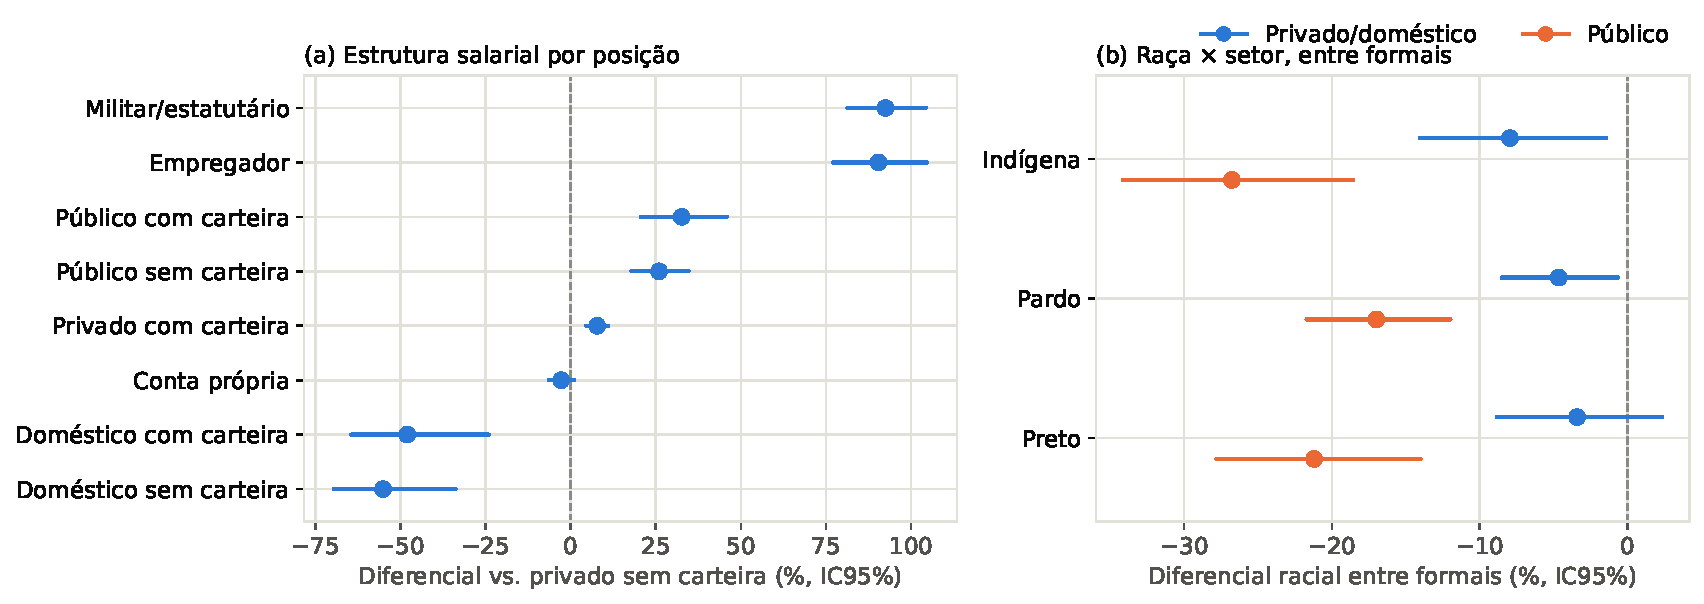
\includegraphics[width=0.88\textwidth]
    {../figures/fig_setor_publico_raca.pdf}
    \caption{Estrutura salarial e diferenciais raciais no setor público}
    \label{fig:raca_setor_publico}
    \begin{minipage}{0.94\textwidth}
    \vspace{0.2cm}
    \scriptsize
    \textit{Nota:} O painel (a) apresenta diferenciais condicionais de
    rendimento por hora segundo posição na ocupação, tendo empregado privado
    sem carteira como referência. O painel (b) apresenta, entre trabalhadores
    formais, os diferenciais de pretos, pardos e indígenas em relação aos
    brancos nos setores privado/doméstico e público. Barras representam
    intervalos de confiança de 95\%. Estimações incorporam o desenho amostral
    da PNAD Contínua e as réplicas bootstrap oficiais.
    \end{minipage}
\end{figure}

O maior \textit{gap} racial observado entre formais não parece, portanto,
constituir uma característica homogênea da formalidade, estando fortemente
associado à composição institucional do segmento formal em Roraima,
especialmente ao setor público. A evidência é compatível com \citet{gerard2021},
mas a PNAD Contínua não permite distinguir de maneira suficientemente fina
carreiras, órgãos, níveis de governo ou funções. Os resultados não permitem,
assim, separar diferenças de remuneração dentro de posições observadas de
\textit{sorting} para carreiras e postos públicos não observados.

\subsection{Sobreposição entre gênero e raça/cor}
\label{subsec:interseccionalidade}

A interação entre gênero e raça/cor mostra que as desvantagens não se combinam
de forma simplesmente aditiva. Em relação aos homens brancos, homens pretos,
pardos e indígenas apresentam diferenciais condicionais de aproximadamente
$-9,6\%$, $-9,2\%$ e $-12,8\%$, e mulheres pretas e pardas, de $-21,5\%$ e
$-22,0\%$. Esses valores são ligeiramente menores em magnitude do que os que
seriam obtidos pela soma aditiva dos componentes de gênero e raça, mas as
respectivas interações não são estatisticamente diferentes de zero. Para
indígenas, o padrão é mais marcado: mulheres indígenas apresentam rendimento por
hora aproximadamente 19,3\% inferior ao de homens brancos observacionalmente
comparáveis, enquanto uma combinação puramente aditiva implicaria diferença
próxima de 28,2\%. A interação mulher$\times$indígena corresponde a
aproximadamente $+12,3\%$ e é estatisticamente significativa ($p=0,004$). As
mulheres indígenas permanecem, portanto, em posição relativa desfavorável, mas
rejeita-se a hipótese de que os diferenciais de gênero e pertencimento indígena
se somem de forma simplesmente aditiva na escala logarítmica. Esse padrão difere
da desvantagem interseccional particularmente intensa encontrada por
\citet{kolev2015} para o Peru e reforça a importância de tratar a categoria
indígena separadamente no contexto roraimense. Como nos demais exercícios, a
interação descreve heterogeneidade condicional e não identifica um mecanismo
causal.

\section{Robustez}
\label{sec:robustez}

Os resultados principais utilizam apenas os quartos trimestres de 2016 a 2025,
opção que busca preservar a comparabilidade sazonal entre os cortes e reduzir
a intensidade de reutilização das unidades amostrais. Para verificar se essa
escolha determina os achados, a especificação principal é reestimada utilizando
todos os trimestres disponíveis no período, com efeitos fixos de
ano$\times$trimestre. A amostra passa, nesse exercício, para 95.198
observações com rendimento válido. Adicionalmente, são consideradas
especificações para 2016--2019, 2022--2025 e para o período completo excluindo
2020 e 2021, de forma a avaliar a sensibilidade dos resultados aos anos da
pandemia.

A Tabela~\ref{tab:robustez_temporal} apresenta os principais coeficientes da
parametrização de referência. Como o modelo contém interações, esses
coeficientes devem ser lidos em relação às categorias de referência. O
coeficiente de formalidade corresponde ao diferencial entre trabalhadores
formais e informais para homens brancos, o coeficiente de mulher corresponde
ao diferencial mulher--homem entre trabalhadores informais brancos e os
coeficientes raciais comparam pretos, pardos e indígenas a brancos entre
homens informais. Os contrastes médios utilizados na interpretação substantiva
da Seção~\ref{sec:resultados} permanecem, portanto, preferíveis para caracterizar
os diferenciais médios, enquanto a tabela permite avaliar diretamente a
estabilidade dos parâmetros estimados.

\begin{table}[htbp]
\centering
\caption{Robustez temporal dos coeficientes da especificação principal}
\label{tab:robustez_temporal}
\scriptsize\singlespacing
\begin{tabular}{lccccc}
\toprule
 & Q4 2016--2025
 & Todos os trimestres
 & 2016--2019
 & 2022--2025
 & Excl. 2020--2021 \\
\midrule

Formal
& 0,295***
& 0,267***
& 0,250***
& 0,276***
& 0,269*** \\
&(0,029)
&(0,014)
&(0,040)
&(0,043)
&(0,028) \\[0.3em]

Mulher
& -0,194***
& -0,184***
& -0,151***
& -0,201***
& -0,181*** \\
&(0,026)
&(0,012)
&(0,041)
&(0,038)
&(0,028) \\[0.3em]

Formal $\times$ Mulher
& -0,005
& 0,018**
& 0,021
& -0,032
& -0,008 \\
&(0,019)
&(0,009)
&(0,030)
&(0,033)
&(0,022) \\[0.3em]

Preto
& -0,101***
& -0,103***
& -0,087*
& -0,056
& -0,065** \\
&(0,030)
&(0,017)
&(0,047)
&(0,042)
&(0,032) \\[0.3em]

Pardo
& -0,096***
& -0,077***
& -0,100***
& -0,101***
& -0,099*** \\
&(0,024)
&(0,012)
&(0,036)
&(0,029)
&(0,022) \\[0.3em]

Indígena
& -0,137***
& -0,132***
& -0,160***
& -0,136**
& -0,151*** \\
&(0,040)
&(0,020)
&(0,060)
&(0,056)
&(0,042) \\

\midrule
N
& 23.938
& 95.198
& 10.267
& 9.922
& 20.189 \\
\bottomrule
\end{tabular}

\vspace{0.15cm}
\begin{minipage}{0.97\textwidth}
\scriptsize
\textit{Nota:} Coeficientes das equações de log do rendimento real por hora;
erros-padrão entre parênteses. Categorias de referência: homem, branco e
informal. Todas as especificações
incluem idade, idade ao quadrado, escolaridade e células
ocupação$\times$atividade. A especificação principal inclui efeitos fixos de
período; a estimação com todos os trimestres utiliza efeitos fixos de
ano$\times$trimestre. Erros-padrão e inferência incorporam o peso amostral e
os pesos de replicação bootstrap oficiais da PNAD Contínua.
$^{***}p<0,01$, $^{**}p<0,05$, $^{*}p<0,10$.
\end{minipage}
\end{table}

A comparação entre as duas primeiras colunas mostra que a ampliação da base
para todos os trimestres produz alterações relativamente pequenas nos
coeficientes. O parâmetro de formalidade passa de 0,295 para 0,267, enquanto
o coeficiente associado às mulheres varia de $-0,194$ para $-0,184$. Entre os
coeficientes raciais, as mudanças também são moderadas. O coeficiente de preto passa de
$-0,101$ para $-0,103$, pardo de $-0,096$ para $-0,077$ e indígena de
$-0,137$ para $-0,132$. Assim, a utilização exclusiva dos quartos trimestres
não parece produzir a direção ou a ordem de magnitude dos principais
resultados.

Os recortes relacionados à pandemia conduzem à mesma conclusão geral. Os
coeficientes de formalidade permanecem positivos e estatisticamente
significativos em todas as especificações, enquanto o diferencial associado
às mulheres permanece negativo e substantivo. Os coeficientes de pardos e
indígenas também conservam sinal e ordem de magnitude. Para pretos, a
estimativa é menos precisa no período 2022--2025 e deixa de ser
estatisticamente diferente de zero, indicando maior incerteza para esse grupo
quando a amostra é fragmentada. Não se observa, contudo, uma reversão
sistemática dos principais resultados entre os períodos pré e pós-pandemia.

A interação entre formalidade e gênero também ilustra a importância de
distinguir estabilidade substantiva de significância pontual dos parâmetros.
Embora o coeficiente seja pequeno e não significativo na especificação
principal, torna-se positivo e estatisticamente significativo quando todos os
trimestres são utilizados, voltando a ser impreciso nos demais recortes.
Como mostrado na Seção~\ref{subsec:resultados_genero}, entretanto, a
interpretação substantiva do diferencial de gênero baseia-se nos contrastes
médios que combinam os termos relevantes da especificação, e não na leitura
isolada desse coeficiente de interação. A oscilação, portanto, reforça a opção
por contrastes como medida principal.

Como verificação adicional, estimam-se tendências lineares mediante interações
entre ano e as variáveis de interesse diretamente no microdado. Não se detecta
tendência linear estatisticamente significativa no diferencial associado à
formalidade ($-0,31\%$ ao ano; $p=0,413$), no diferencial feminino
($-0,34\%$; $p=0,245$), no de pretos ($+0,67\%$; $p=0,307$) ou no de
indígenas ($+0,78\%$; $p=0,340$). Para pardos, estima-se redução do
diferencial de aproximadamente 0,96\% ao ano ($p=0,022$). A evidência de
convergência temporal é, portanto, restrita a esse grupo e não caracteriza um
movimento generalizado dos diferenciais ao longo de 2016--2025.

Em conjunto, os exercícios indicam que os principais resultados não dependem
do uso exclusivo dos quartos trimestres nem parecem ser produzidos pelos anos
da pandemia. As magnitudes variam entre recortes, como esperado em um mercado
de pequena escala e com algumas células amostrais reduzidas, mas a estrutura
central dos achados permanece. A formalidade está associada a maior rendimento,
o diferencial feminino permanece negativo após condicionamento e os
diferenciais raciais persistem, ainda que com maior imprecisão para alguns
grupos. Esses resultados reforçam a estabilidade descritiva das associações
estimadas, sem alterar sua interpretação não causal.

\section{Considerações finais}
\label{sec:conclusao}

Este artigo investigou como formalidade, gênero e raça/cor se associam aos
diferenciais de rendimento em Roraima entre 2016 e 2025. A formalidade
permanece associada a maiores rendimentos após controles extensos, embora o
diferencial diminua quando a análise é restrita às relações de emprego,
resultado compatível com a heterogeneidade da informalidade documentada pela
literatura \citep{curi2006, meghir2015, ulyssea2018}.

A principal contribuição do artigo está em mostrar que composição observável e
formalidade operam de maneira distinta para gênero e raça/cor. Entre mulheres,
um diferencial bruto de rendimento por hora praticamente nulo torna-se uma
desvantagem condicional próxima de 15\%, sendo a escolaridade a principal
dimensão associada a essa mudança, em linha com \citet{giuberti2005}. Para
raça/cor, os elevados \textit{gaps} brutos caem substancialmente após o controle
pela escolaridade, indicando que desigualdades acumuladas antes da comparação
salarial respondem por parcela importante da desvantagem racial
\citep{soares2000, campante2004}. Essas diferenças de composição não eliminam,
contudo, os diferenciais dentro do mercado de trabalho. Mulheres permanecem com
rendimento por hora inferior ao dos homens tanto entre formais quanto entre
informais, e os diferenciais raciais condicionais permanecem negativos e têm
estimativas pontuais maiores no segmento formal, com diferença estatisticamente
clara apenas para indígenas.

No caso de Roraima, a centralidade do setor público é fundamental para
compreender esse resultado, pois a maior magnitude dos \textit{gaps} raciais
entre trabalhadores formais está fortemente concentrada no emprego público. Em
um mercado no qual o Estado possui peso particularmente elevado como empregador,
a heterogeneidade institucional documentada pela literatura sobre o setor
público \citep{foguel2000, moriconi2009, mattos2022, baez2021} também pode ser
relevante para a estrutura das desigualdades raciais. A separação da categoria
indígena, por sua vez, revela os maiores diferenciais entre os grupos raciais e
mostra que gênero e pertencimento indígena não se acumulam de forma
simplesmente aditiva, embora mulheres indígenas continuem apresentando
rendimento inferior ao de homens brancos comparáveis, o que reforça a
importância de evitar agregações raciais amplas. Além disso, a jornada responde
por parcela importante do diferencial mensal de gênero, enquanto os
\textit{gaps} raciais são predominantemente associados à remuneração por hora.

Essas conclusões devem ser interpretadas dentro dos limites do desenho
empírico. As estimações não identificam efeitos causais da formalidade, do
emprego público, do gênero ou da raça/cor, e os diferenciais condicionais podem
incorporar características produtivas não observadas, alocação entre firmas,
carreiras e níveis de governo e mecanismos discriminatórios que a PNAD Contínua
não permite isolar. Ainda assim, o caso de Roraima mostra que estimativas
nacionais podem ocultar combinações específicas entre estrutura produtiva,
presença estatal e composição demográfica, e que compreender a desigualdade em
mercados regionais exige ir além da dicotomia formal--informal. Bases que
permitam acompanhar trajetórias individuais e identificar firmas, carreiras
públicas e níveis de governo constituem uma extensão natural desta agenda.

\begingroup
\normalsize
\section{Declaração sobre uso de Inteligência Artificial}

Ferramentas de inteligência artificial foram utilizadas como apoio à programação, 
formatação, organização e revisão do manuscrito. Claude (Anthropic) e ChatGPT
(OpenAI) auxiliaram na elaboração e depuração de rotinas em R e Python; na formatação 
do documento; e no planejamento, estruturação e revisão textual. 
Todos os códigos, resultados e conteúdos foram revisados e validados pelos autores, 
que assumem integral responsabilidade pelo artigo.

\endgroup

\begingroup
\small\singlespacing
\setlength{\bibsep}{6pt}
\bibliographystyle{chicago-pt}
\bibliography{../referencias}
\endgroup

\end{document}
